\chapter{Scan Konvertierung / Clipping}

\section{Clipping}

Wenn man in einem Raum auf ein Objekt schaut, so sieht man nur z.B. nur einen Teil davon. Der andere Teil wäre schon da, ist aber nicht sichtbar. In einer 3D Rendering Engine wäre es jetzt unnötig, dazu alle Lichteffekt usw. schon zu berechnen, deswegen schneidet man es weg. Das nennt man Clipping.

\subsection{3D vs 2D Clipping}
Clipping geschieht in mehreren Stufen. Nachdem die 3D Szene aufgebaut ist, werden 3D Objekte entfernt, welche z.B. nicht im View Bereich der Kamera sind. Das wäre 3D Clipping. 2D Clipping bedeutet, dass nachdem alle Beleuchtung usw. berechnet wurde, noch der Teil rausgeschniten wird, der nicht auf den Bildschirm passt - bevor das Bild dann schlussendlich gerastert und dargestellt wird.
\begin{figure}[!ht]
	\centering
	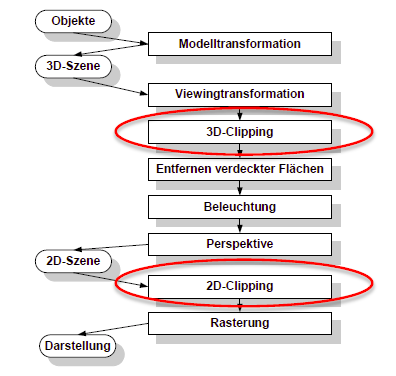
\includegraphics[width=0.4\linewidth]{fig/grafikpipeline}
	\caption{Grafikpipeline}
	\label{fig:grafikpipeline}
\end{figure}

\subsection{Clipping Variationen}
Man kann auf verschiedene Arten allgemein nun Clippen (3D).
\begin{enumerate}
	\item \textbf{Scissering} \\
	Die 'dümmste' Variante des Clippings. Hier wird das 3D Clipping einfach übersprungen und nur am Schluss einfach die gezeichnet, welche gerade so im Fenster liegen.
	\item \textbf{Temporärer Buffer} \\
	Das gesamte Objekt wird in einem temporären Buffer gezeichnet, welcher anschliessend kopiert wird. (Anmk. des Autors - keine Ahnung was das ist. Bitte um Hilfe.)
	\item \textbf{Analytische Berechnung} \\ 
	Man berechnet irgendwie, was darin liegt. Man siehe unten.
\end{enumerate}

\subsection{Linien Clipping}
Gehen wir von einem ganz einfachen Fall aus - dem Clipping einer Linie. Wir haben also ein Rechteck, welches z.B. den Canvas darstellt. Hindurch geht eine Linie. Wir möchten nun berechnen, welche Punkte gezeichnet werden müssen, resp. eine Linie haben, welche genau innerhalb des gezeichneten Rechtecks ist. Dazu gibt es die nachfolgenden Varianten.

\subsubsection{Brute Force}
Wenn mindestens ein Endpunkt der Linie ausserhalb des Rechtecks liegt (also wenn die Linie einfach etwas herausgeht aus dem Rechteck), dann müsste man alle Schnittpunkte berechnen, die die Linie mit dem Kappungs-Rechteck hat. Das scheint aber für CG Anwendungen zu unperformant zu sein.

\subsubsection{Cohen-Sutherland}
Nette Herren, die sich folgende Methode ausgedacht haben:
\begin{enumerate}
	\item Nimm den Anfangs- \& Endpunkt der Linie. Schau, in welchem Bereich der Punkt liegt:
	
	\begin{figure}[!ht]
		\centering
		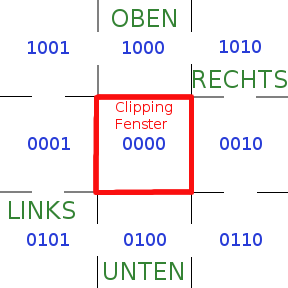
\includegraphics[width=0.3\linewidth]{fig/cohen_sutherland}
		\caption{Bereiche der Grafik für den Algorithmus von Cohen Sutherland}
		\label{fig:cohen_sutherland}
	\end{figure}
	
	Liegt der Punkt oben rechts vom Clipping Fenster, so hat der Punkt den Wert \textit{1010}. Ist er rechts unten, so ist der Wert \textit{0110}. Der Wert wird also bitweise bestimmt, in der Reihenfolge:
	\begin{enumerate}
		\item Oben (1000)
		\item Unten (0100)
		\item Rechts (0010)
		\item Links (0001)
	\end{enumerate}
	\item Ist der Code bei beiden Punkten \textit{0000}, so liegen ja beide Punkte im Clipping Fenster und die Linie wird akzeptiert und so gezeichnet.
	\item Ansonsten wird Bit für Bit der Wert verglichen und geschaut, ob bei beiden der Wert 1 ist. Das heisst es wird das erste Bit genommen, dann das zweite usw. Eigentlich wird geschaut, ob beide Punkte links, rechts, oben oder unten des Rechtsecks sind. Denn wenn das der Fall ist, so geht die Linie nämlich sicher nicht durch das Clipping Fenster und die Linie kann abgelehnt werden.
	\item Wenn die Linie aber durch das Vergleichen nicht abgelehnt werden konnte, so wird der Schnittpunkt mit einer beliebigen Seite des Clipping Fensters berechnet und die Linie so \textit{entzweigeschnitten}. Einen Teil der Linie kann dann verworfen werden, der andere Teil der Linie wird nochmals durch den Algorithmus gejagt, bis dann alles im Rechteck vorhanden ist.
\end{enumerate}

\subsection{Polygone Clippen}
Das wird schon etwas aufwändiger. Wir haben hier einen Algorithmus von den Herren \textbf{Sutherland-Hodgeman}, der eigentlich nur für Geraden geht - aber da ein Rechteck ja eigentlich einfach aus 4 Geraden besteht, machen wir das Ganze einfach 4x - dann passts auch.

Ein Polygon besteht ja aus n-Punkten. Wir gehen jetzt von einem Startpunkt aus und gehen dann von Punkt zu Punkt. Wir schauen dann jeweils einfach für den Startpunkt \textit{S} und den nächsten Punkt des Polygons \textit{P}, ob diese Punkte innerhalb oder ausserhalb des Polygons liegen. Dies wird für alle Punkte gemacht, das heisst jeder Punkt ist mal Startpunkt und jeder Punkt ist mal Endpunkt. Die Ausgabe des Algorithmus bestimmt dann, welcher Punkt behalten wird. Wenn die Punkte die Linien schneiden, wird einfach der Schnittpunkt dazu berechnet und entsprechend auch gespeichert.
	
	\begin{figure}[!ht]
		\centering
		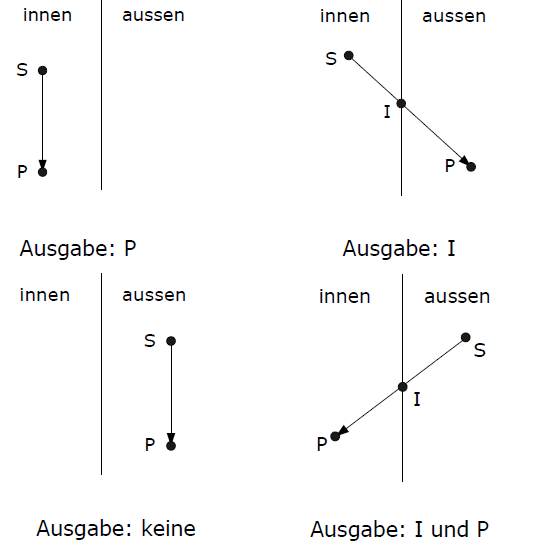
\includegraphics[width=0.5\linewidth]{fig/sutherland_hodgman}
		\caption{Verschiedene Fälle für den Sutherland Hodgman Algorithmus}
		\label{fig:sutherland_hodgman}
	\end{figure}

\section{Visibility}
Es geht darum, unsichtbare Flächen nicht darstellen zu lassen - sonst sieht es ja komisch aus.

\subsection{Backface Culling}
Wenn die Objekte geschlossen sind, dann kann einfach der Normalenvektor der Fläche betrachtet werden - denn wenn ein Vektor wegzeigt muss diese Fläche liegt dann ja auf der Rückseite und muss logischerweise nicht gezeichnet werden.

\subsection{Tiefensortierung}
Sortiere die Polygone und zeichne sie dann von hinten nach vorne, sodass die zuletzt gezeichneten Polygone die anderen überdecken. Wird auch als \textit{Maleralgorithmus} bezeichnet.
\subsubsection{Vorteile}
\begin{enumerate}
	\item Auch für transparente Objekte möglich
	\item Einfach für Spezialfälle
\end{enumerate}
\subsubsection{Nachteile}
\begin{enumerate}
	\item Ineffizient für viele Objekte \(O(n^2)\)
	\item Wird nicht direkt Hardware unterstützt
	\item Nicht für jedes Objekt direkt möglich - unpassende Objekte  müssen z.B. noch weiter zerschnitten werden
\end{enumerate}
\subsubsection{Details}
Im Detail sieht das dann so aus:
Von jedem Polygon wird der Punkt genommen, der am nächsten zur Kamera ist. Anhand dieser Entfernen werden die Polygone zuerst einmal grob sortiert. Wenn jetzt sich irgendwo Polygone überschneiden, also z.B. Polygon A ist zwischen 2 und 10 von der Kamera entfernt und Polygon B zwischen 8 und 11, dann wird noch weiteres gemacht.

Polygon A ist zur Zeit jetzt ja näher bei der Kamera. Falls nun irgend eine folgende Bedingung zutrifft, werden sie nicht vertauscht, ansonsten schon.

\begin{enumerate}
	\item \textbf{Überlagern sich die x-Ausdehnungen nicht?} \\
	Auf gut Deutsch: Sind die Objekte vollständig nebeneinander?
	\item \textbf{Überlagern sich die y-Ausdehnungen nicht?} \\
	Sind die Objekte vollständig hintereinander? Abbildung \ref{fig:ausdehnungen} zeigt ein Beispiel, wo die Objekte vollständig nebeneinander sind, aber nicht vollständig hintereinander.
		\begin{figure}[!ht]
			\centering
			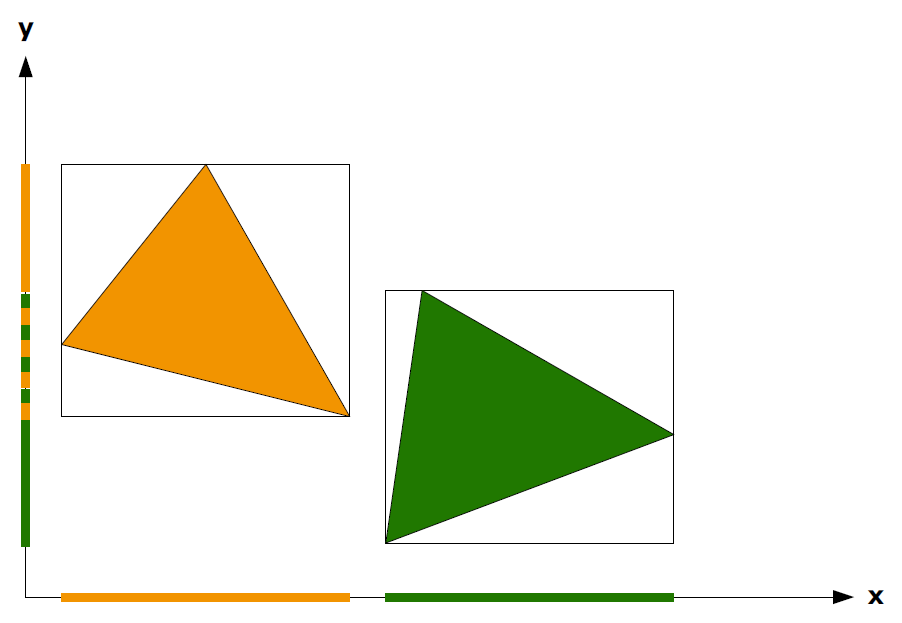
\includegraphics[width=0.5\linewidth]{fig/ausdehnungen}
			\caption{Beispiel Ausdehnung von 2 Objekten}
			\label{fig:ausdehnungen}
		\end{figure}
	\item \textbf{Liegt das hintere Objekt ganz auf der vom Betrachter abgewandeten Seite vom vorderen Objekt?} \\
	Kein Plan was das bedeuteten soll.
		\begin{figure}[!ht]
			\centering
			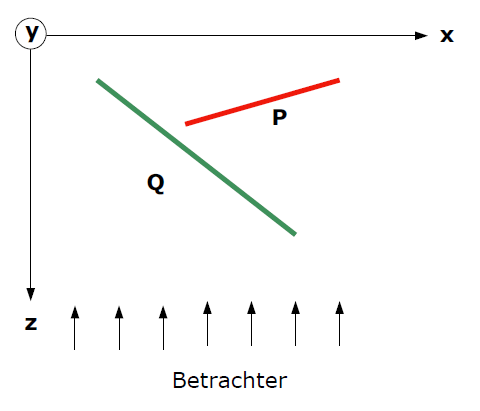
\includegraphics[width=0.5\linewidth]{fig/tiefensortierung_3}
			\caption{Ein Beispiel dazu}
			\label{fig:tiefensortierung_3}
		\end{figure}
	\item \textbf{Liegt das vordere Objekt komplett auf der Betrachterseite vom vorderen Objekt?}\\
		\begin{figure}[!ht]
			\centering
			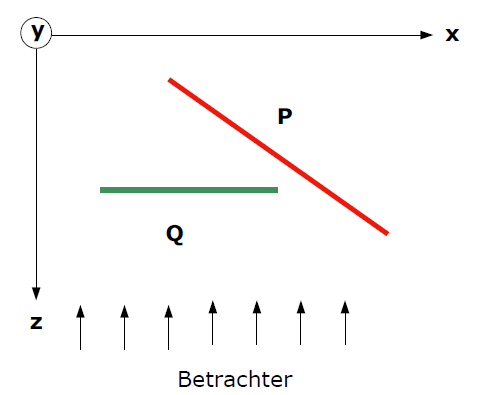
\includegraphics[width=0.5\linewidth]{fig/tiefensortierung_4}
			\caption{Ein Beispiel dazu}
			\label{fig:tiefensortierung_4}
		\end{figure}
	\item \textbf{Überlappen sich die Polygone nicht auf der Projektion in die xy Ebene?}\\
		\begin{figure}[!ht]
			\centering
			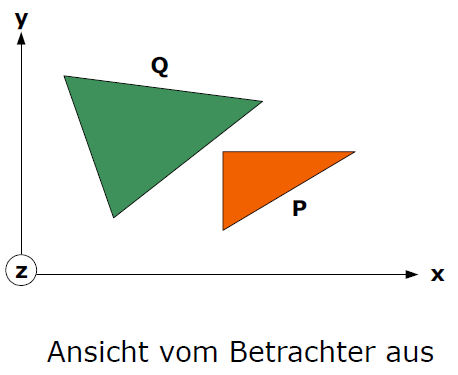
\includegraphics[width=0.5\linewidth]{fig/tiefensortierung_5}
			\caption{Ein Beispiel dazu}
			\label{fig:tiefensortierung_5}
		\end{figure}
	Nehmen wir an, die beiden Objekte sind die zwei Dreiecke - wenn wir jetzt stur von vorne auf diese Objekte schauen, sind diese ja 2-Dimensional. Wenn sich diese nicht schneiden, wie im Beispiel in Abbildung \ref{fig:tiefensortierung_5}, dann ist diese Bedingung erfüllt.
	
\end{enumerate}
\subsection{Z Buffer}
Auf Grund der Nachteile vom Tiefensortieren hat man einen ganz einfachen Algorithmus entwickelt. Dieser zeichnet alle Polygone, berechnet also die R, G und B Werte und zusätzlich noch die Entfernung zur Kamera - der Z Wert. Beim Zeichnen der Pixel wird dann einfach geprüft, ob der aktuelle Pixel näher ist.
\subsubsection{Vorteile}
\begin{enumerate}
	\item Hardwareunterstützt
	\item Polygone können in beligiger Reihenfolge gezeichnet werden
	\item Zeitkomplexität ist O(n), aber häufig sogar konstant ab einer gewissen Anzahl Polygone.
\end{enumerate}
\subsubsection{Nachteile}
\begin{enumerate}
	\item Rundungsprobleme
	\item Was ist, wenn zwei Pixel denselben z Wert haben? (Dann gibts Artefakte vom überlappen)
	\item (grosser Speicherbedarf - heute nicht mehr soo problematisch)
\end{enumerate}
\subsubsection{Berechnung von z}
Z lässt sich aus der Ebenengleichung berechnen
\begin{displaymath}
	z = \frac{-D-Ax-By}{C}
\end{displaymath}
oder inkrementell entlang einer Scanlinie
\begin{displaymath}
	z_{neu} = \frac{-D-A(x_{alt}+1)-By}{C}=z_{alt}-\frac{A}{C}
\end{displaymath}
\subsection{Warnock Algorithmus}
Hier wird der Bildbereich angeschaut und entschieden, ob er \textit{einfach} zu zeichnen ist. Ist er das nicht, wird er in 4 Unterbereiche unterteilt, für welche dann wieder einzeln entschieden wird, ob sie \textit{einfach} sind. Das ist dementsprechend rekursiv.
\subsubsection{Einfache Bereiche}
Ein Bereich ist einfach, falls...
\begin{enumerate}
	\item ... er kein oder nur 1 Polygon enthält.
	\item ... nur ein Polygon beinhaltet, das am nächsten ist und den Bereich auch vollständig füllt.
	\item ... er nur 1 Pixel gross ist.
\end{enumerate}
\begin{figure}[!ht]
	\centering
	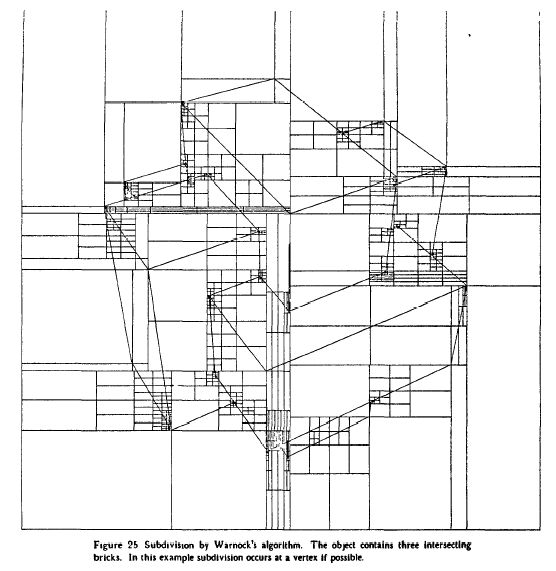
\includegraphics[width=0.5\linewidth]{fig/warnock}
	\caption{Ein Beispiel zu Warnock}
	\label{fig:warnock}
\end{figure}
\subsection{Various}
Ein Ausdehnungsbereich ist ein möglichst kleines Rechteck (Bounding Box), welches das Objekt vollständig enthält. Wenn sich solche Ausdehnungsbereiche nicht schneiden, so schneiden sich logischerweise auch die Objekte nicht.\\
Objektraum = alle Objekte\\
Bildraum = alle Pixel